\section{Networking on the Pi}
\label{sec:NetworkingOnThePi}
There are many ways to interface with the Pi. This section will cover types of network connectivity.

\subsection{A Brief Overview of Networks}
\label{app:UnderstandingNetworks}
It is useful to have a basic idea of how networks, IP addresses, and subnets work. For this, it it suggested you read \href{https://support.microsoft.com/en-za/help/164015/understanding-tcp-ip-addressing-and-subnetting-basics}{this article} from Microsoft: \href{https://tinyurl.com/y2z8x9za}{https://tinyurl.com/y2z8x9za}

\subsection{Assigning a Static IP to the Pi}
\label{sec:Connectivity-Ethernet}
This section will assign a static Ethernet address to the Raspberry Pi. This is useful for your first configuration. If you have not done so, it is recommended you follow the instructions in Section\ref{sec:Installation} to configure your Raspberry Pi.
\begin{enumerate}
    \item Insert the SD card into your computer and navigate to the BOOT partition
    \item Open "cmdline.txt" and append the following to the line (don't create a new line)
        \begin{lstlisting}[gobble=8]
        ip=192.168.137.15
        \end{lstlisting}
        This tells the Raspberry Pi to configure the Ethernet port to use the IP address 192.168.137.15
    \item Enable SSH as per Section \ref{sec:SSH}.
    \item You need to configure your PC to use the same subnet as the Pi. To do so, see the information below in Section \ref{sec:Connectivity-ChangeComputerIP}
\end{enumerate}

\subsection{Assigning a Static IP to your Computer}
In order to use Ethernet for SSH, VNC, etc, it is required that the Pi and your computer all be on the same subnet. This section details how to do it.
\label{sec:Connectivity-ChangeComputerIP}
\subsubsection{Windows}
To change the IP of your Ethernet port on Windows 10, complete the following steps:
\begin{itemize}
    \item Right click on your network option in Windows taskbar
    \item Select"Open Network \& Internet Settings", on the lower right hand side of the screen.
    \item Select "Change Adapted Options"
    \item Right click on the Ethernet Connection and select "Properties"
    \item Select "Internet Protocol Version 4 (TCP/IPv4) and click "Properties"
    \item Select "Use the following IP address:" and enter in the following options:\\
            - IP Address: 192.168.137.1\\
            - Subnet Mask: 255.255.255.0
    \item You have successfully changed the IP of the Ethernet card on your computer. It is suggested that you now ensure connectivity by attempting to ping the Pi.
\end{itemize}

\begin{figure}[H]
\centering
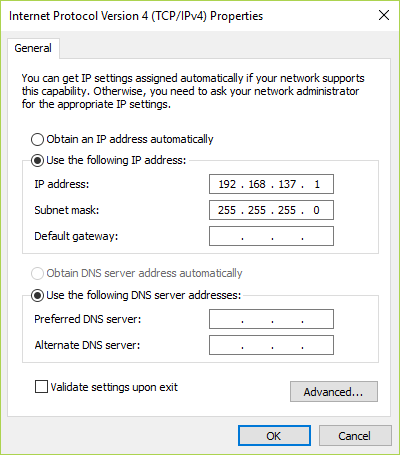
\includegraphics[width=0.6\columnwidth]{Figures/WindowsIPConfig}
\caption{The IPv4 configuration screen in Windows 10}
\label{fig:WindowsIPConfig}
\end{figure}


\subsubsection{Ubuntu}
To change the IP of your Ethernet port on Ubuntu, complete the following steps:
\begin{itemize}
    \item Click the network interface icon on the status bar and select Wired Settings
    \item Click the gear button of the interface you'd like to change
    \item Select the IPv4 Tab, and change the IPv4 method to Manual
    \item Under "Addresses" enter in the following:\\
            - IP Address: 192.168.137.1\\
            - Subnet Mask: 255.255.255.0
    \item You can leave Gateway and DNS blank
\end{itemize}

\begin{figure}[H]
\centering
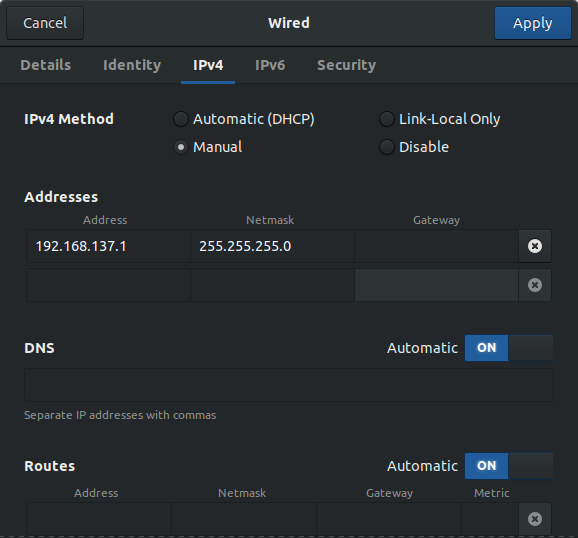
\includegraphics[width=0.6\columnwidth]{Figures/ubuntustaticip}
\caption{The IPv4 configuration screen in Ubuntu 18.10}
\label{fig:ubuntustaticip}
\end{figure}

\subsection{Ensuring connectivity}
\label{sec:Connectivity-EnsuringConnectivity}
Sometimes you may want to debug your connection to the Pi. A fast way to do this is via the \textit{ping} command. \textit{Ping} sends a packet to a particular host (in this case the Pi), and measures the time taken for a response from that host. 

To use the ping command, open a command prompt window or terminal and type the following:
\begin{lstlisting}
$ ping 192.168.137.15
\end{lstlisting}

If that host is unreachable (the Pi hasn't booted yet or is incorrectly configured), a message will show that the host is unreachable. If everything was correctly configured, you should get
\begin{lstlisting}
Reply from 192.168.137.15: bytes=32 time<1ns TTL=64
\end{lstlisting}

This means your Pi and computer are both correctly configured. See section \ref{sec:SSH} for configuring your Pi for SSH access.

\textbf{NB:} Don't be surprised if you can't ping a Windows machine from your Pi. Windows blocks the specific type of packet required for a ping in the firewall.